\documentclass[10pt,twocolumn,letterpaper]{article}

\usepackage{cvpr}
\usepackage{times}
\usepackage{epsfig}
\usepackage{graphicx}
\usepackage{amsmath}
\usepackage{amssymb}


\usepackage{booktabs}
\usepackage[table]{xcolor}

% Include other packages here, before hyperref.

% If you comment hyperref and then uncomment it, you should delete
% egpaper.aux before re-running latex.  (Or just hit 'q' on the first latex
% run, let it finish, and you should be clear).
\usepackage[pagebackref=true,breaklinks=true,letterpaper=true,colorlinks,bookmarks=false]{hyperref}


%%%%%%%%%%%%%%
\newcommand{\C}{{\cal C}}
\newcommand{\D}{{\cal D}}
\newcommand{\Y}{{\cal Y}}
\newcommand{\X}{{\cal X}}
\newcommand{\R}{{\cal R}}
\renewcommand{\H}{{\cal H}}
\renewcommand{\S}{{\cal S}}
\newcommand{\bm}[1]{\boldsymbol{#1}}
\newcommand{\argmax}{\ensuremath{\mathop{\mathrm{argmax}}}}

\newcommand{\thetav}{\ensuremath{\bm{\theta}}}

\newcommand{\specialcell}[2][c]{\begin{tabular}[#1]{@{}c@{}}#2\end{tabular}}

\def\be {\begin{equation}}
\def\ee {\end{equation}}
\def\beas {\begin{eqnarray*}}
\def\eeas {\end{eqnarray*}}
\def\bea {\begin{eqnarray}}
\def\eea {\end{eqnarray}}
\def\bes {\begin{equation*}}
\def\ees {\end{equation*}}
\def\ba {\begin{align}}
\def\ea {\end{align}}
\def\barr {\begin{array}}
\def\earr {\end{array}}

\def\tran {\top}

\newtheorem{theorem}{Theorem}
\newtheorem{proposition}{Prop}
\newtheorem{lemma}{Lemma}
\newtheorem{lemma-ap}{Lemma}
\newtheorem{definition}{Definition}
\newtheorem{corollary}{Corollary}
\newtheorem{claim}{Claim}
\newtheorem{claim-ap}{Claim}
\newtheorem{program}{Program}
\newtheorem{property}{Property}

\makeatletter

\usepackage{xspace}
\def\@onedot{\ifx\@let@token.\else.\null\fi\xspace}
\DeclareRobustCommand\onedot{\futurelet\@let@token\@onedot}

\newcommand{\figref}[1]{Fig\onedot~\ref{#1}}
\newcommand{\equref}[1]{Eq\onedot~\eqref{#1}}
\newcommand{\secref}[1]{Sec\onedot~\ref{#1}}
\newcommand{\tabref}[1]{Tab\onedot~\ref{#1}}
\newcommand{\thmref}[1]{Theorem~\ref{#1}}
\newcommand{\prgref}[1]{Program~\ref{#1}}
%\newcommand{\algref}[1]{Alg\onedot~\ref{#1}}
\newcommand{\clmref}[1]{Claim~\ref{#1}}
\newcommand{\lemref}[1]{Lemma~\ref{#1}}
\newcommand{\ptyref}[1]{Property\onedot~\ref{#1}}

\newcommand{\fix}{\marginpar{FIX}}
\newcommand{\new}{\marginpar{NEW}}

\newcommand{\by}[2]{\ensuremath{#1 \! \times \! #2}}

\def\eg{\emph{e.g}\onedot} \def\Eg{\emph{E.g}\onedot}
\def\ie{\emph{i.e}\onedot} \def\Ie{\emph{I.e}\onedot}
\def\cf{\emph{cf}\onedot} \def\Cf{\emph{Cf}\onedot}
\def\etc{\emph{etc}\onedot} \def\vs{\emph{vs}\onedot}
\def\wrt{w.r.t\onedot} \def\dof{d.o.f\onedot}
\def\etal{\emph{et al}\onedot}

%%%%%%%%% PAPER ID  - PLEASE UPDATE
\def\cvprPaperID{2195} % *** Enter the CVPR Paper ID here
\def\httilde{\mbox{\tt\raisebox{-.5ex}{\symbol{126}}}}

\begin{document}

%%%%%%%%% TITLE - PLEASE UPDATE
\title{Attention to Scale: Scale-aware Semantic Image Segmentation}  % **** Enter the paper title here

\maketitle
\thispagestyle{empty}


%%%%%%%%% BODY TEXT - ENTER YOUR RESPONSE BELOW

\section{Rebuttal}
\label{sec:overview}
\vspace{-0.17cm}
We thank all reviewers for their valuable comments. We start our rebuttal by summarizing our contributions and then address each reviewer's comments.
%We first summarize the paper and then address each reviewer's comments.

Attention models have shown a great success in several computer vision and natural language processing tasks by allowing the model to focus on the most relevant features.
%One of the most curious facets of the human visual system is the presence of attention (Rensink, 2000; Corbetta \& Shulman, 2002).
%Rather than compressing an entire image or sequence into a static representation,
%attention allows the model to focus on the most relevant features as needed.
Unlike current works employing the attention model in the 2D spatial and/or temporal dimension, we explore its effect in the scale dimension.
%While all previous works focus on 2D spatial and temporal dimension, we study the effect on the scale dimension which is not addressed in the computer vision literature before.
%The concept of scale here is an encoding of both object depth and semantic scale, corresponding to the weighted selection of feature pyramids that best recognizes objects at different scales.
%The idea behind this is that to recognize objects at different scales, CNN image receptive field size should vary at different pixel locations.
%The observation behind is that human changes pupil focal length when looking at different objects.
%The key contribution of this paper is the scale-attention model for semantic image segmenation, which seems not been addressed in the computer vision literature before.
%The proposed attention model is no more complicated than the fully-convolutional models and is able to utilize multi-scale image features efficiently.
To the best of our knowledge, no other published work explores attention in this dimension. % for the task of semantic image segmentation.

Specifically, we show that the improvement of proposed whole model is {\it accumulated} by (1) multi-scale inputs (2) extra supervision and (3) attention model. The proposed model significantly improves over baseline DeepLab-LargeFOV (\eg, 6.4\% on PASCAL test set), and yields significantly better performance than DeepLab-MSc variants (\eg, 4.5\% on PASCAL test set) while only one-step {\it end-to-end} training is required. It also gives non-trivial 1\% improvement over average- or max-pooling methods.
Most importantly, the proposed attention model provides diagnostic visualization, unveiling the black box operation of average- or max-pooling by visualizing the weight (\ie, importance of features) at each scale for every position.

\vspace{-0.17cm}
\subsection{Reviewer 1}
\vspace{-0.17cm}
Q: ... use more scales in training ...

A: We have explored four scales \{1, 0.75, 0.5, 0.25\} in our analysis experiments on PASCAL-Person-Part, and found that the performance of average-pooling drops around 0.5\% while max-pooling and attention model have similar performance as three scales \{1, 0.75, 0.5\} (\ie, more robust to noisy scales). We think the scale {0.25} produces too small score maps after VGG-16 net.  As suggested, we further explore more scales \{1, 0.875, 0.75, 0.675, 0.5\} on PASCAL VOC 2012, but we do not observe any improvement over using three scales \{1, 0.75, 0.5\} (attention model still better by 1\%). Our image pyramid does not contain scale larger than one, similar to the pyramid employed by Deformable Parts Model \cite{felzenszwalb2010object}.
%, as upsampling may induce noisy interpolation values (similar to DPM \cite{felzenszwalb2010object}).

Q: ... why a joint training is necessary.

A: Training the attention model independent of the segmentation network requires the supervision of ``scale'' of each pixel. However, it is both tedious and difficult to accurately annotate the ground truth scale for each pixel. Furthermore, the input scale quantization error (it is infeasible to enumerate all possible scales) makes it more reasonable to assign soft weights to each pixel. The problems are ameliorated by the proposed joint training, letting the model adaptively find the best weights on scales
for each pixel.

Q: ... theoretical guarantee ... attention model ... worse.

A: Attention models are proven useful in several areas (\eg, machine translation) most empirically, instead of theoretically. In Tab. 3, attention model (71.52\%) attains better mIOU than average- (70.53\%) and max-pooling (70.58\%, just {\it uploaded}), and it is better in 17 categories.

Q: How ... extra supervision is implemented ...

A: In addition to the supervision to the final merged output, we inject extra supervision to the output (\ie, fc8) of DeepLab for each scale. Considering the case w/ two input scales, the total loss function contains three cross entropy loss functions (one for final output and one for each scale) with weight one for each. The ground truths are downsampled properly \wrt. the output resolutions during training.

Q: .. unclear ... generalized to datasets with larger scale

A: The proposed model works well for the person class on MS-COCO which contains large scale variation.
%A: As discussed in the paper, the person class in the MS-COCO dataset contains large scale variation, and our proposed method generalizes well for it.

%% Q: ... proposed method ... not better from recent works.

%% A: Our models are trained end-to-end with one pass to exploit multi-scale features. State-of-art models usually require multiple training stages (\eg, four stages in [27]).

Q: implementation ... complicated ... hard to generalize

A: The implementation of attention model is not complicated since it only consists of two convolutional layers. The slicing operation of the weight maps from attention model is the slice\_layer in CAFFE. Conceptually, the weighting operation for each scale input can be implemented by ``repmat'' in MATLAB since $w_i^s$ in Eq. (1) is shared across all channels. How to handle multi-scale properly is an important issue in computer vision and we think the proposed whole model is one step towards solving it. The effectiveness of our model has been shown on three datasets. %Our proposed method generalizes well, as we have observed similar trend on three challenging datasets.

%% \begin{table}[t!]
%%   \centering
%%   \begin{tabular}{c}
%%   \centering
%%   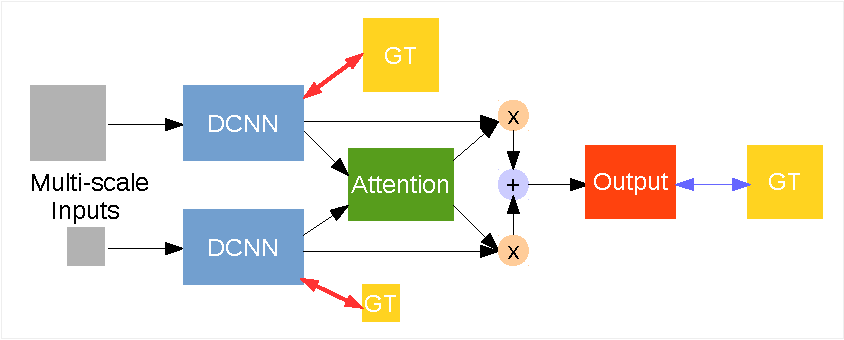
\includegraphics[width=0.8\linewidth]{fig/extra_sup_2.pdf}
%%   \end{tabular}
%%   \caption{Illustration of adding extra supervision. Added extra supervision is shown by the red arrows.}
%%   \label{fig:extra_sup}
%% \end{table}


%% \begin{table*}[b!] %\scriptsize
%% %\rowcolors{2}{}{ultramarineblue!35}
%% \setlength{\tabcolsep}{3pt}
%% \resizebox{2.1\columnwidth}{!}{
%% \begin{tabular}{l||c||c*{20}{|c}}
%% \toprule[0.2 em]
%% Method         & mean & bkg &  aero & bike & bird & boat & bottle& bus & car  &  cat & chair& cow  &table & dog  & horse & mbike& person& plant&sheep& sofa &train & tv  \\
%% \midrule \midrule
%% \href{http://host.robots.ox.ac.uk:8080/anonymous/OBB7IY.html}{DeepLab-LargeFOV-{\bf AveragePooling}} & 70.5 & 92.7 & 83.5 & 37.2 & 75.4 & 60.9 & 69.3 & 89.0 & 83.4 & 83.5 & 28.2 & 73.4 & 58.7 & 78.4 & 79.0 & 83.0 & 79.7 & 54.4 & 79.6 & 50.2 &
%% 78.0 & 63.5 \\
%% \href{http://host.robots.ox.ac.uk:8080/anonymous/1TQ8XB.html}{DeepLab-LargeFOV-{\bf MaxPooling}} & 70.6 & 92.7 & 84.1 & 37.7 & 75.7 & 62.2 & 69.2 & 89.0 & 83.6 & 84.5 & 28.0 & 73.9 & 59.5 & 79.7 & 77.3 & 82.1 & 80.0 & 53.8 & 79.9 & 50.3 & 76.3 & 62.6 \\
%% \href{http://host.robots.ox.ac.uk:8080/anonymous/1TN3OK.html}{DeepLab-LargeFOV-{\bf Attention}} & 71.5 & 92.9 & 86.0 & 38.8 & 78.2 & 63.1 & 70.2 & 89.6 & 84.1 & 82.9 & 29.4 & 75.2 & 58.7 & 79.3 & 78.4 & 83.9 & 80.3 & 53.5 & 82.6 & 51.5 & 79.2 & 64.2  \\
%% \midrule
%%  \end{tabular}
%% }
%%  \caption{Labeling IOU on the PASCAL VOC 2012 test set, using the trainval set for training.}
%%  \label{tab:voc2012_rebuttal}
%% \end{table*}

\vspace{-0.17cm}
\subsection{Reviewer 2}
\vspace{-0.17cm}
Q: ... variant DeepLab-MSc missing

A: We explore DeepLab-MSc variants combined with proposed methods on three datasets and do not observe significant improvement (\eg, on VOC-12 val set, DeepLab-MSc-LargeFOV-Attention has performance 67.13\%, lower than DeepLab-LargeFOV-Attention 69.08\%). Besides, DeepLab-MSc variants requires a two-step training process (first DeepLab backbone is trained and then side output classifier), which is not as efficient as proposed models.

%Q: ... unclear ... generalize to other ... systems
%A: DeepLab is a variant of FCN; thus, we think it generalizes well to other segmentation systems.

Q: ... replace max-pooling layers ... by attention model.

A: This is an interesting future work. The main issue is how to efficiently perform pooling (by attention model) over both spatial positions and scales. % (current proposed method only perform element-wise pooling over scales).

\vspace{-0.17cm}
\subsection{Reviewer 3}
\vspace{-0.17cm}
Q: ... improvement is too small to convince ...

A: Please see \secref{sec:overview} above. We emphasize that the proposed model outperforms DeepLab-MSc-LargeFOV in {\bf 20} categories (only except bike) in Tab. 3.

\vspace{-0.17cm}
{\scriptsize
\bibliographystyle{ieee}
\bibliography{egbib}
}
\vspace{-0.17cm}

\end{document}
